\documentclass[11pt,a4paper]{article}

% Csomagok
\usepackage[utf8]{inputenc}
\usepackage[magyar]{babel}
\usepackage[margin=2cm]{geometry}
\usepackage{graphicx}
\usepackage{booktabs}
\usepackage{longtable}
\usepackage{xcolor}
\usepackage{colortbl}
\usepackage{tikz}
\usepackage{pgfplots}
\usepackage{fancyhdr}
\usepackage{multicol}
\usepackage{tcolorbox}
\usepackage{fontawesome5}

\pgfplotsset{compat=1.17}

% Színek definiálása
\definecolor{clgreen}{HTML}{66CC66}
\definecolor{clblue}{HTML}{6699FF}
\definecolor{clred}{HTML}{FF6666}
\definecolor{clyellow}{HTML}{FFCC66}
\definecolor{clgray}{HTML}{CCCCCC}

% Fejléc/lábléc
\pagestyle{fancy}
\fancyhf{}
\lhead{Premier League - 10. forduló}
\rhead{2024/25}
\cfoot{\thepage}

% Címoldal adatok
\title{
    \Huge \textbf{Premier League} \\
    \Large 2024/25 Szezon \\
    \large 10. Forduló Összefoglaló
}
\author{}
\date{2025. November 27.}

\begin{document}

% ==================== CÍMOLDAL ====================
\maketitle
\thispagestyle{empty}

\begin{center}
\Large Időszak: 2024-11-02 -- 2024-11-04
\end{center}

\vfill

\begin{center}
\textit{Automatikusan generált riport}
\end{center}

\newpage

% ==================== EXECUTIVE SUMMARY ====================
\section*{Executive Summary}

\begin{tcolorbox}[colback=blue!5,colframe=blue!40,title=Főbb Insights]
\begin{itemize}
    \item Manchester City kiváló formában: 2.6 forma-index, 1. helyezés
\end{itemize}
\end{tcolorbox}

\vspace{1em}

% ==================== TABELLA & MOMENTUM ====================
\section*{Aktuális Tabella}

\begin{longtable}{clccccccl}
\toprule
\textbf{Hely} & \textbf{Csapat} & \textbf{M} & \textbf{Gy} & \textbf{D} & \textbf{V} & \textbf{Pont} & \textbf{GK} & \textbf{Forma} \\
\midrule
\endhead

        \rowcolor{green!30}
    1 & 
    Manchester City & 
    10 & 
    7 & 
    2 & 
    1 & 
    \textbf{23} & 
    17 & 
    WWDWW \\
        \rowcolor{green!30}
    2 & 
    Arsenal & 
    10 & 
    6 & 
    3 & 
    1 & 
    \textbf{21} & 
    12 & 
    WDWDW \\
        \rowcolor{green!30}
    3 & 
    Liverpool & 
    10 & 
    6 & 
    2 & 
    2 & 
    \textbf{20} & 
    9 & 
    WLWWD \\
        \rowcolor{green!30}
    4 & 
    Chelsea & 
    10 & 
    5 & 
    3 & 
    2 & 
    \textbf{18} & 
    6 & 
    DWWDW \\
    14 & 
    Manchester United & 
    10 & 
    3 & 
    2 & 
    5 & 
    \textbf{11} & 
    -5 & 
    LLWDL \\
\bottomrule
\end{longtable}

\begin{small}
\textcolor{clgreen}{\faSquare} Bajnokok Ligája \quad
\textcolor{clblue}{\faSquare} Európa Liga \quad
\textcolor{cyan}{\faSquare} Konferencia Liga \quad
\textcolor{clred}{\faSquare} Kiesőzóna
\end{small}

\vspace{1em}

\subsection*{Momentum - Pozícióváltozások}

\begin{center}
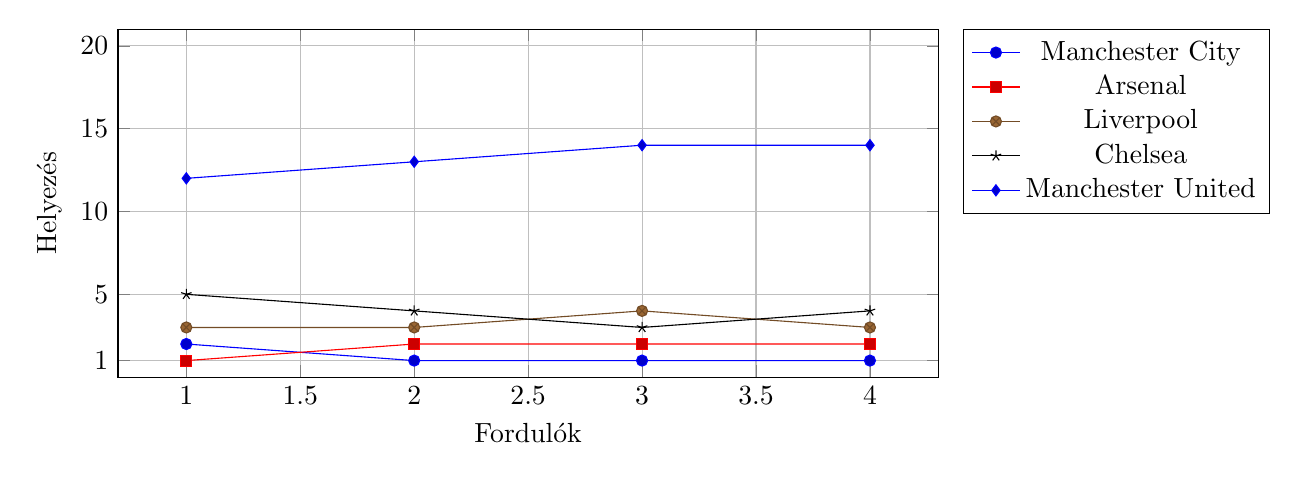
\begin{tikzpicture}
\begin{axis}[
    width=12cm,
    height=6cm,
    xlabel={Fordulók},
    ylabel={Helyezés},
    ymin=0, ymax=21,
    ytick={1,5,10,15,20},
    legend pos=outer north east,
    grid=major
]

    \addplot coordinates {
        (1, 2)
        (2, 1)
        (3, 1)
        (4, 1)
    };
    \addlegendentry{Manchester City}
    \addplot coordinates {
        (1, 1)
        (2, 2)
        (3, 2)
        (4, 2)
    };
    \addlegendentry{Arsenal}
    \addplot coordinates {
        (1, 3)
        (2, 3)
        (3, 4)
        (4, 3)
    };
    \addlegendentry{Liverpool}
    \addplot coordinates {
        (1, 5)
        (2, 4)
        (3, 3)
        (4, 4)
    };
    \addlegendentry{Chelsea}
    \addplot coordinates {
        (1, 12)
        (2, 13)
        (3, 14)
        (4, 14)
    };
    \addlegendentry{Manchester United}
\end{axis}
\end{tikzpicture}
\end{center}

\newpage

% ==================== FORDULÓ EREDMÉNYEK ====================
\section*{10. Forduló Eredményei}

\begin{center}
\begin{tabular}{lclccc}
\toprule
\textbf{Hazai} & & \textbf{Vendég} & \textbf{Eredmény} & \textbf{xG} & \textbf{Típus} \\
\midrule

    Manchester City & vs & Arsenal & 
    2:1 & 
    1.8 - 1.2 &
        --
    \\
    Liverpool & vs & Chelsea & 
    1:1 & 
    2.1 - 0.9 &
        --
    \\
    Manchester United & vs & West Ham & 
    0:2 & 
    0.8 - 2.3 &
        --
    \\
\bottomrule
\end{tabular}
\end{center}

\vspace{1em}

\begin{tcolorbox}[colback=yellow!10,colframe=yellow!50,title=\faStar~ Meglepetés Eredmények]
\end{tcolorbox}

\newpage

% ==================== STATISZTIKAI TOPLISTÁK ====================
\section*{Statisztikai Toplista}

\begin{multicols}{2}

\subsection*{\faChartLine~ Top 5 Támadás}
\begin{tabular}{lc}
\toprule
\textbf{Csapat} & \textbf{xG} \\
\midrule
    Manchester City & 23.5 \\
    Arsenal & 20.8 \\
    Liverpool & 19.2 \\
    Chelsea & 17.5 \\
    Manchester United & 14.8 \\
\bottomrule
\end{tabular}

\vspace{1.5em}

\subsection*{\faChartLine~ Top 5 Védelem}
\begin{tabular}{lc}
\toprule
\textbf{Csapat} & \textbf{xGA} \\
\midrule
    Manchester City & 7.2 \\
    Arsenal & 9.5 \\
    Liverpool & 11.8 \\
    Chelsea & 13.2 \\
    Manchester United & 15.2 \\
\bottomrule
\end{tabular}

\columnbreak

\subsection*{\faFire~ Legjobb Forma}
\begin{tabular}{lc}
\toprule
\textbf{Csapat} & \textbf{Index} \\
\midrule
    Manchester City & 2.6 \\
    Chelsea & 2.3 \\
    Arsenal & 2.2 \\
    Liverpool & 1.95 \\
    Manchester United & 0.85 \\
\bottomrule
\end{tabular}

\vspace{1.5em}

\subsection*{\faArrowDown~ Legrosszabb Forma}
\begin{tabular}{lc}
\toprule
\textbf{Csapat} & \textbf{Index} \\
\midrule
    Manchester United & 0.85 \\
    Liverpool & 1.95 \\
    Arsenal & 2.2 \\
    Chelsea & 2.3 \\
    Manchester City & 2.6 \\
\bottomrule
\end{tabular}

\end{multicols}

\vspace{1em}

\subsection*{Teljesítmény-rés (Pont vs xPoints)}

\begin{center}
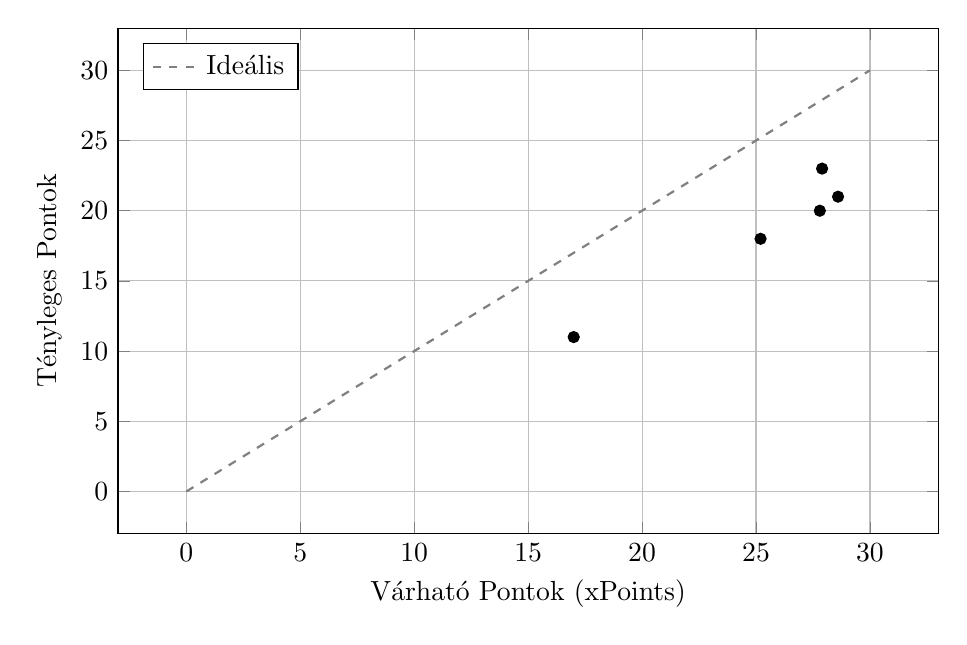
\begin{tikzpicture}
\begin{axis}[
    width=12cm,
    height=8cm,
    xlabel={Várható Pontok (xPoints)},
    ylabel={Tényleges Pontok},
    grid=major,
    legend pos=north west
]

% Referencia vonal (ideális teljesítmény)
\addplot[dashed, thick, gray] coordinates {(0,0) (30,30)};
\addlegendentry{Ideális}

% Csapatok
    \addplot[only marks, mark=*, mark size=2pt] 
    coordinates {(27.9, 23)};
    \addplot[only marks, mark=*, mark size=2pt] 
    coordinates {(28.6, 21)};
    \addplot[only marks, mark=*, mark size=2pt] 
    coordinates {(27.8, 20)};
    \addplot[only marks, mark=*, mark size=2pt] 
    coordinates {(25.2, 18)};
    \addplot[only marks, mark=*, mark size=2pt] 
    coordinates {(17.0, 11)};
\end{axis}
\end{tikzpicture}
\end{center}

\newpage

% ==================== TRENDANALÍZIS ====================
\section*{Trendanalízis \& Figyelmeztetések}

\subsection*{\faArrowUp~ Felfelé Ívelő Csapatok}

\begin{tcolorbox}[colback=green!5,colframe=green!40]
\end{tcolorbox}

\subsection*{\faExclamationTriangle~ Veszélyzóna}

\begin{tcolorbox}[colback=red!5,colframe=red!40]
\end{tcolorbox}

\subsection*{Alul/Felülteljesítők}

\begin{multicols}{2}

\textbf{Felülteljesítők} (szerencsések):
\begin{itemize}
    \item Manchester City: +-4.9 pont
    \item Manchester United: +-6.0 pont
    \item Chelsea: +-7.2 pont
\end{itemize}

\columnbreak

\textbf{Alulteljesítők} (szerencsétlenek):
\begin{itemize}
    \item Liverpool: -7.8 pont
    \item Arsenal: -7.6 pont
    \item Chelsea: -7.2 pont
\end{itemize}

\end{multicols}

\newpage

% ==================== KÖVETKEZŐ FORDULÓ ====================
\section*{Következő Forduló Előzetes}

\subsection*{\faCalendar~ Top Mérkőzések}

    \begin{tcolorbox}[colback=blue!5,colframe=blue!30]
    \textbf{Arsenal vs Liverpool} \\
    \textit{Dátum:} 2024-11-09 \\
    \textit{Nehézség:} 8.5/10 \\
    \textit{Kontextus:} Tabellaszomszédok csatája - Bajnoki Liga helyért
    \end{tcolorbox}
    \vspace{0.5em}
    \begin{tcolorbox}[colback=blue!5,colframe=blue!30]
    \textbf{Chelsea vs Manchester City} \\
    \textit{Dátum:} 2024-11-09 \\
    \textit{Nehézség:} 9.0/10 \\
    \textit{Kontextus:} Címvédő elleni rangadó
    \end{tcolorbox}
    \vspace{0.5em}
    \begin{tcolorbox}[colback=blue!5,colframe=blue!30]
    \textbf{Manchester United vs Leicester} \\
    \textit{Dátum:} 2024-11-10 \\
    \textit{Nehézség:} 6.0/10 \\
    \textit{Kontextus:} Bennmaradási harc
    \end{tcolorbox}
    \vspace{0.5em}
\vfill

\begin{center}
\rule{0.5\textwidth}{0.4pt} \\
\textit{Generálva: 2025. November 27.} \\
\textit{Automatizált Liga-Összefoglaló Rendszer}
\end{center}

\end{document}